\documentclass[aspectratio=43]{beamer}
\usepackage{ragged2e}
\usepackage{multirow}

\usetheme{CSCS}

\newcommand{\footlinetext}{Summer School 2015 - MPI}

% Select the image for the title page
%\newcommand{\picturetitle}{cscs_images/image3.pdf}
\newcommand{\picturetitle}{cscs_images/image5.pdf}
%\newcommand{\picturetitle}{cscs_images/image6.pdf}

\author{Maxime Martinasso, CSCS}
\title{Message Passing Interface (MPI)}
\subtitle{Summer School 2015 - Effective High Performance Computing}
\date{July 22-23, 2015}

\begin{document}

% TITLE SLIDE
\cscstitle

\begin{frame}{Previous course summary}
\begin{itemize}
\item Point-to-point communication
\item Blocking and non-blocking communication
\item Transfer modes
\end{itemize}
\end{frame}

\begin{frame}{Course Objectives}
\begin{itemize}
\item The understanding of a collective operations
\item Knowledge of the different collective operations
\end{itemize}
\end{frame}

% TABLE OF CONTENT SLIDE
\cscstableofcontents[hideallsubsections]{General Course Structure}

\section{An introduction to MPI}
\section{Point-to-point communications}
\section{Collective communications}
\cscstableofcontents[currentsection]{General Course Structure}

% CHAPTER SLIDE
\cscschapter{Collective communications}

\subsection{Collective communications}

\begin{frame}{Collective operations}
Communications involving a group of processes part of a communicator.
Different algorithms: $1\rightarrow N$, $N\rightarrow 1$ or $N\rightarrow N\;$ ($1\rightarrow 1$ = pt2pt).\\

Example:
\begin{itemize}
\item Barrier Synchronization
\item Broadcast
\item Gather/Scatter
\item AlltoAll
\item Reduction (sum, max, prod, ... )
\end{itemize}

Features:
\begin{itemize}
    \item All processes must call the collective routine, one is the root
    \item No tags
\end{itemize}

The MPI library should use the most efficient communication algorithm for the particular platform.
\end{frame}


\subsection{Barrier}

\begin{frame}[fragile]{Barrier}
Stop processes until all processes within a communicator reach the barrier.\\
\begin{Cpplisting}[]{}
int MPI_Barrier(MPI_Comm comm);
\end{Cpplisting}
\begin{Fortranlisting}[]{}
MPI_BARRIER(comm, ierr)
\end{Fortranlisting}
\begin{center}
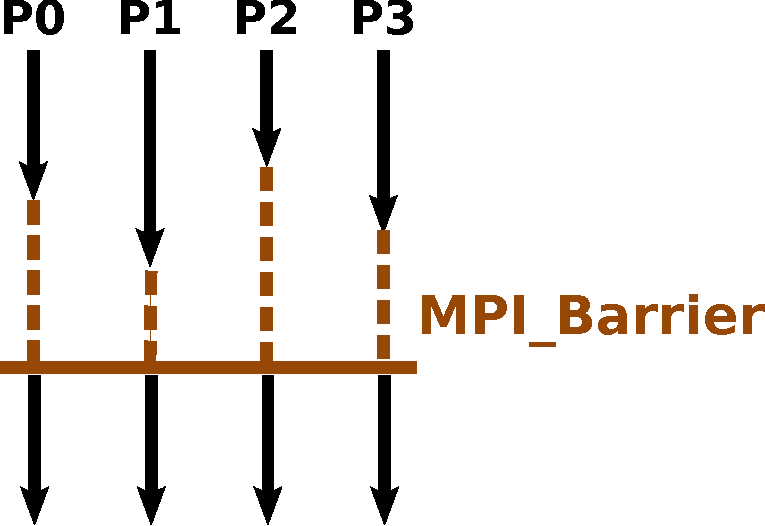
\includegraphics[scale=0.5]{03.MPI_Coll/barrier.pdf}
\end{center}
\end{frame}

\subsection{Broadcast}
\begin{frame}[fragile]{Broadcast}
One-to-all communication: same data sent from root process to all other processes in the communicator.\\
\begin{Fortranlisting}[]{}
CALL MPI_BCAST(buf, count, type, root, comm, ierr)
\end{Fortranlisting}
\begin{black1block}{}
\begin{tabular}{rp{8cm}}
\textbf{root} & (INTEGER) rank being the initiator of the collective operation\\
\end{tabular}
\end{black1block}
\begin{center}
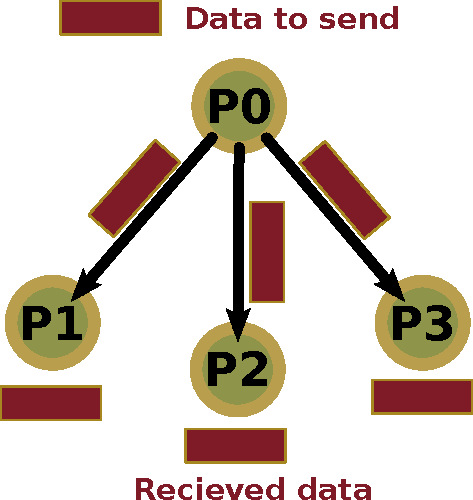
\includegraphics[scale=0.5]{03.MPI_Coll/broadcast.pdf}
\end{center}
\end{frame}

\begin{frame}{Practicals}
\begin{brown2block}{Exercise: 03.MPI\_Coll}
    \begin{enumerate}
        \item Read from the terminal and broadcast the input
    \end{enumerate}
    \end{brown2block}
\end{frame}


\subsection{Scatter/Gather}
\begin{frame}{Scatter and Gather}
\begin{tabular}{c|c}
    \textbf{Scatter} & \textbf{Gather} \\
    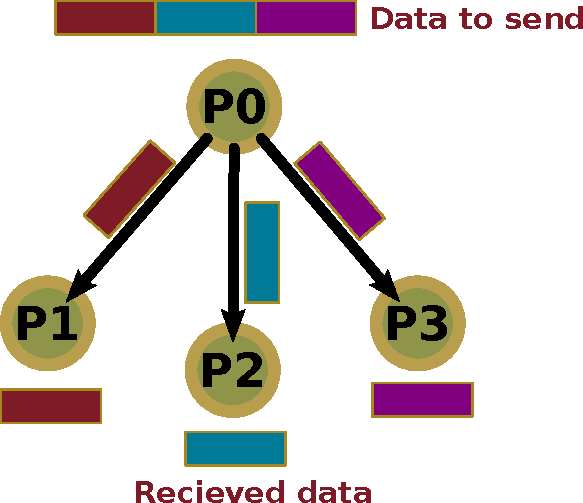
\includegraphics[scale=0.5]{03.MPI_Coll/scatter.pdf} & 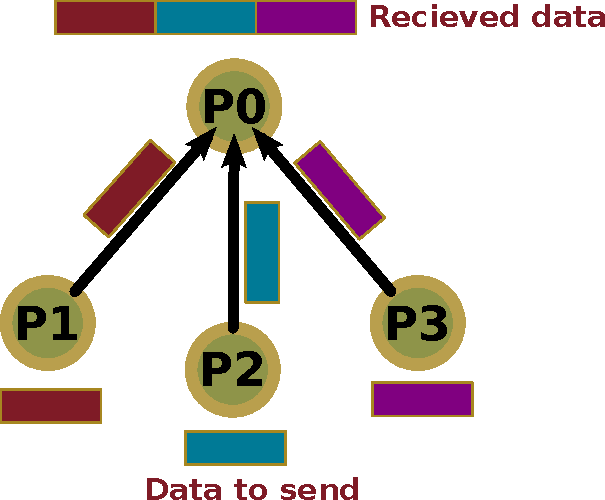
\includegraphics[scale=0.5]{03.MPI_Coll/gather.pdf} \\
\end{tabular}
\end{frame}

\begin{frame}[fragile]{Scatter}
One-to-all communication: different data sent from the root process to all other processes in the communicator.\\
\begin{Fortranlisting}[]{}
CALL MPI_SCATTER(sndbuf, sndcount, sndtype,
                 rcvbuf, rcvcount, rcvtype,
                 root, comm, ierr)
\end{Fortranlisting}
\begin{black1block}{}
\begin{tabular}{rp{8cm}}
\textbf{sndcount} & (INTEGER) number of elements sent to each process, not the size of sndbuf, that should be sndcount times the number of process in the communicator\\
\textbf{rcvcount} & (INTEGER) number of element in the receive buffer\\
\end{tabular}
\end{black1block}
\begin{columns}
    \begin{column}{0.7\paperwidth}
        \hspace{1cm}The sender arguments are meaningful only for root.
    \end{column}
    \begin{column}{0.3\paperwidth}
    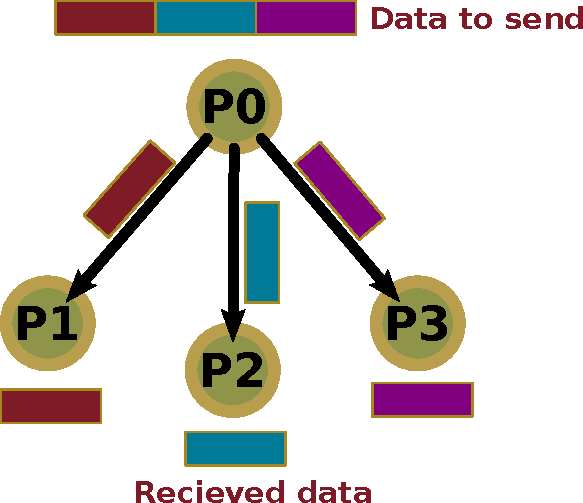
\includegraphics[scale=0.3]{03.MPI_Coll/scatter.pdf}\\
    \end{column}
\end{columns}
\end{frame}

\begin{frame}{Scatter with identical buffer size}
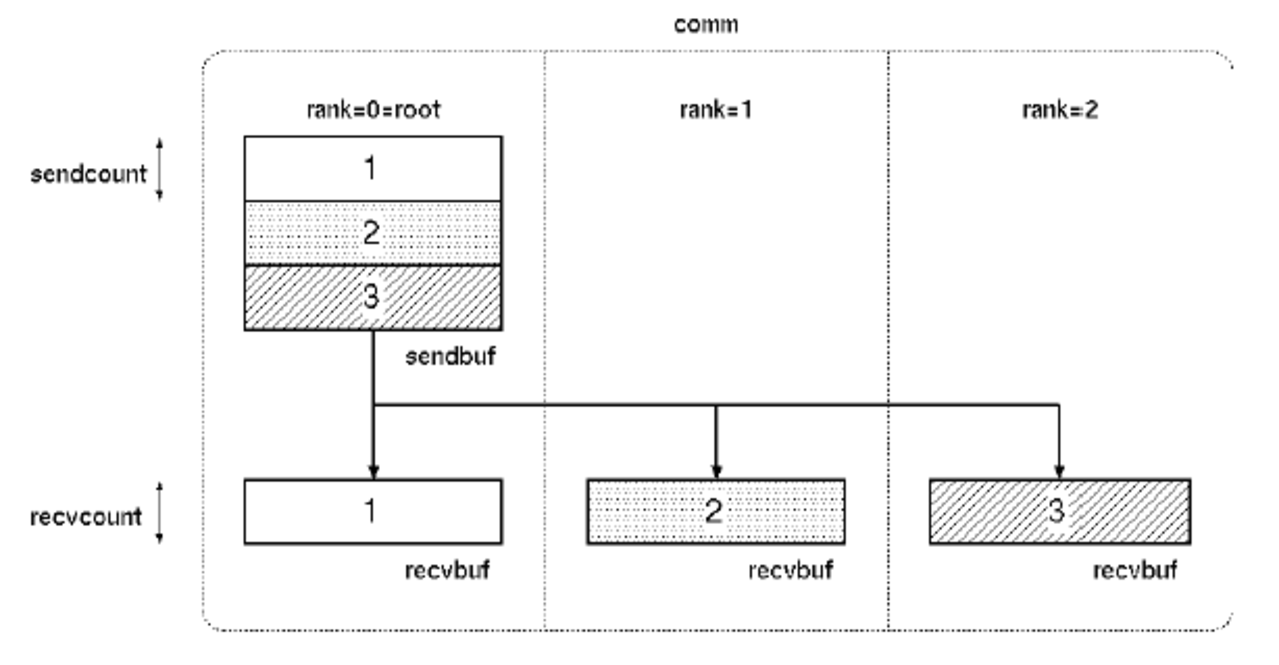
\includegraphics[scale=0.5]{03.MPI_Coll/scatter1.pdf}
\end{frame}

\begin{frame}[fragile]{Scatter with different buffers size}
One-to-all communication: Scatter + distributes individual messages from root to each process in communicator. Messages can have different sizes and displacements.\\
\begin{Fortranlisting}[]{}
CALL MPI_SCATTERV(sndbuf, sndcount, displs, sndtype,
                  rcvbuf, rcvcount, rcvtype,
                  root, comm, ierr)
\end{Fortranlisting}
\begin{black1block}{}
\begin{tabular}{rp{8cm}}
\textbf{displs} & (INTEGER) entry i specifies the displacement (relative to sendbuf) from which to take the outgoing data to process i.\\
\end{tabular}
\end{black1block}
\begin{center}
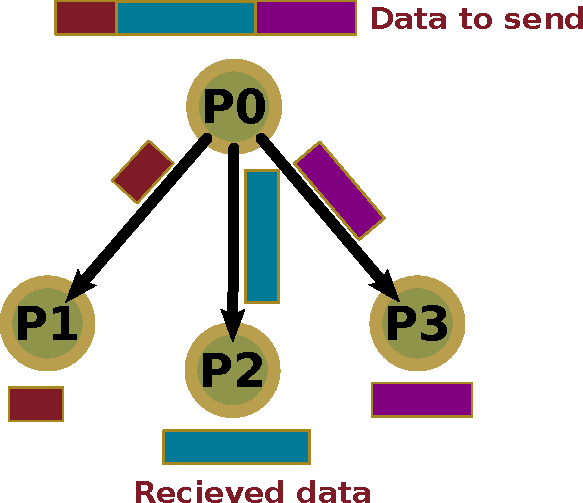
\includegraphics[scale=0.33]{03.MPI_Coll/scatterv.pdf}
\end{center}
\end{frame}

\begin{frame}{Scatter with different buffers size}
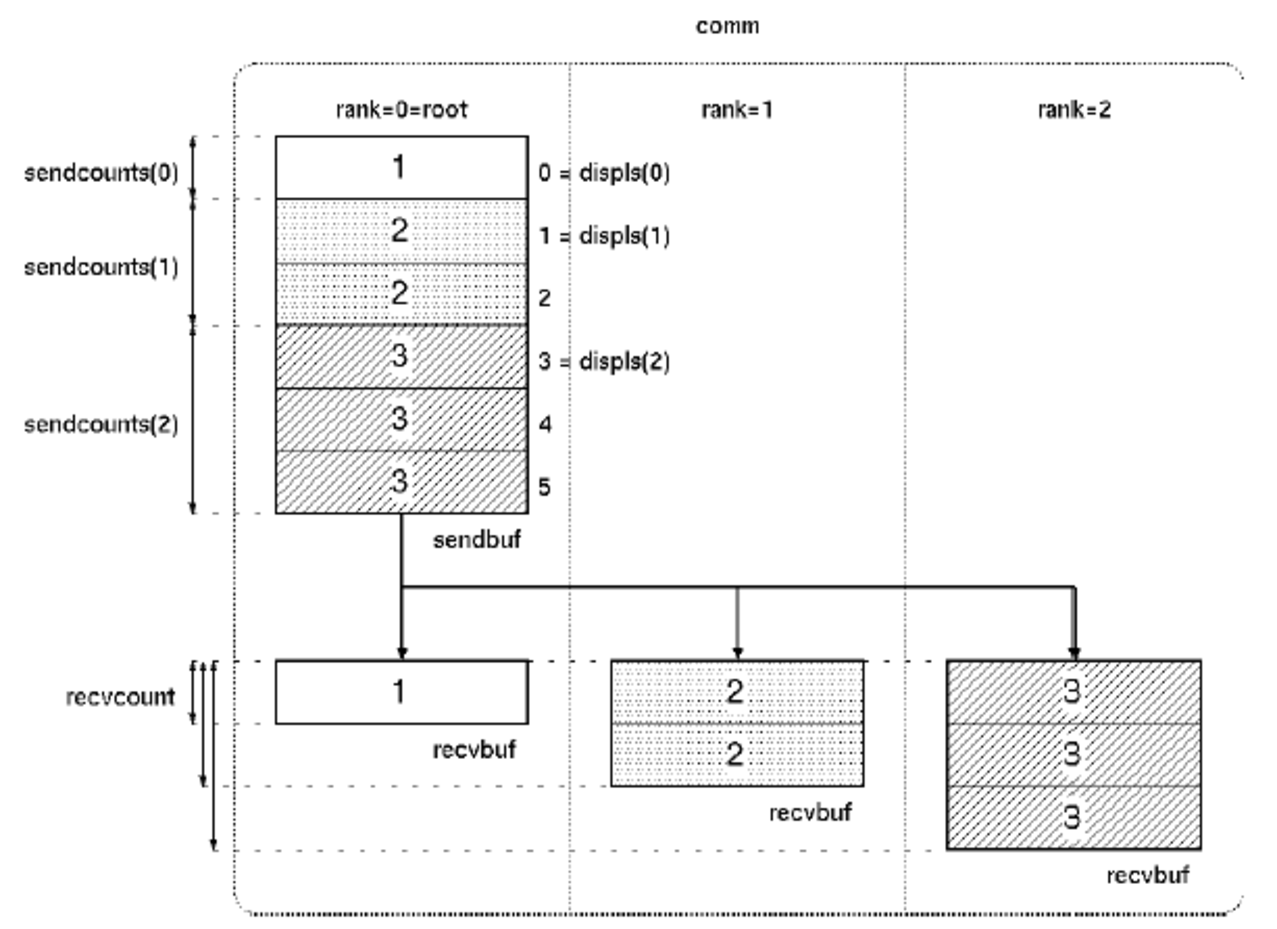
\includegraphics[scale=0.5]{03.MPI_Coll/scatter2.pdf}
\end{frame}

\begin{frame}[fragile]{Gather}
One-to-all communication: different data collected by the root process, from all others processes in the communicator.\\
\begin{Fortranlisting}[]{}
CALL MPI_GATHER(sndbuf, sndcount, sndtype,
                rcvbuf, rcvcount, rcvtype,
                root, comm, ierr)
\end{Fortranlisting}
\begin{black1block}{}
\begin{tabular}{rp{8cm}}
\textbf{rcvcount} & (INTEGER) the number of elements collected from each process, not the size of rcvbuf, that should be rcvcount times the number of process in the communicator\\
\textbf{sndcount} & (INTEGER) number of element in the send buffer\\
\end{tabular}
\end{black1block}
\begin{columns}
    \begin{column}{0.7\paperwidth}
        \hspace{1cm}The receive arguments are meaningful only for root.
    \end{column}
    \begin{column}{0.3\paperwidth}
    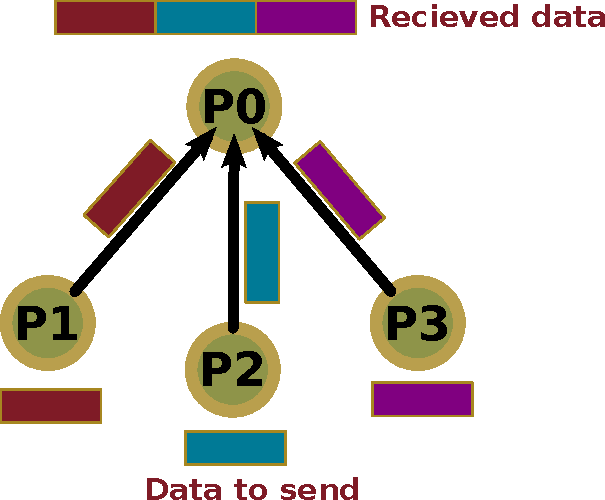
\includegraphics[scale=0.3]{03.MPI_Coll/gather.pdf}\\
    \end{column}
\end{columns}
\end{frame}

\begin{frame}{Gather with identical buffer size}
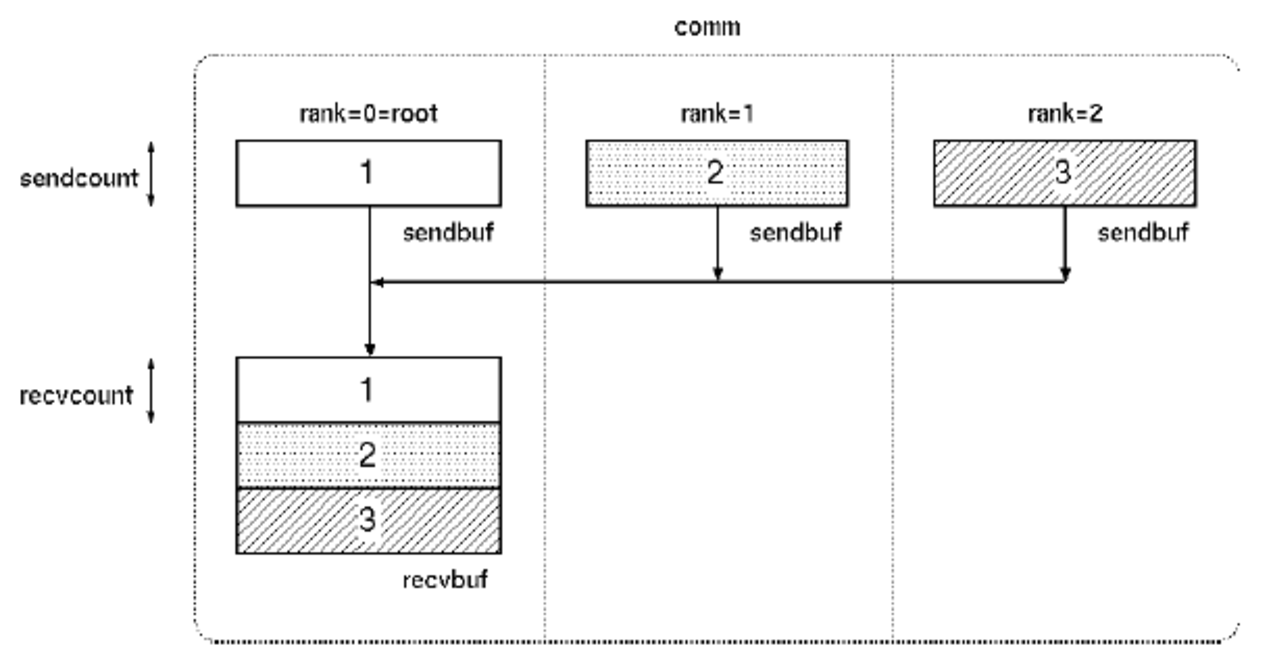
\includegraphics[scale=0.5]{03.MPI_Coll/gather1.pdf}
\end{frame}

\begin{frame}[fragile]{Gather with different buffers size}
One-to-all communication: Gather + collects individual messages from each process in communicator to the root process and store them in rank order. Messages can have different sizes and displacements.\\
\begin{Fortranlisting}[]{}
CALL MPI_GATHERV(sndbuf, sndcount, sndtype,
                 rcvbuf, rcvcount, displs, rcvtype,
                 root, comm, ierr)
\end{Fortranlisting}
\begin{black1block}{}
\begin{tabular}{rp{8cm}}
\textbf{displs} & (INTEGER) entry i specifies the displacement (relative to sendbuf) from which to take the outgoing data to process i.\\
\end{tabular}
\end{black1block}
\begin{center}
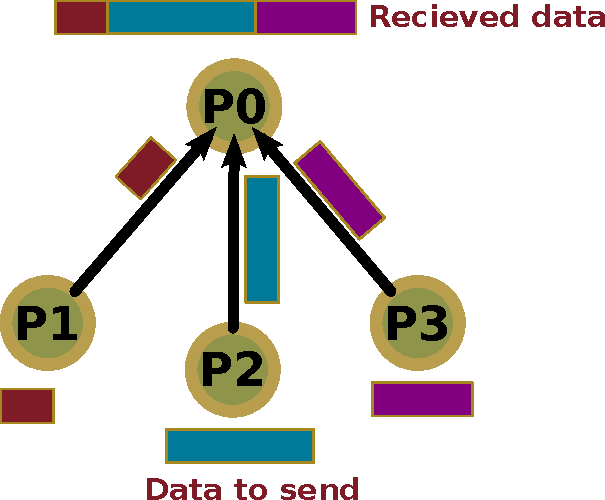
\includegraphics[scale=0.33]{03.MPI_Coll/gatherv.pdf}
\end{center}
\end{frame}

\begin{frame}{Gather with different buffers size}
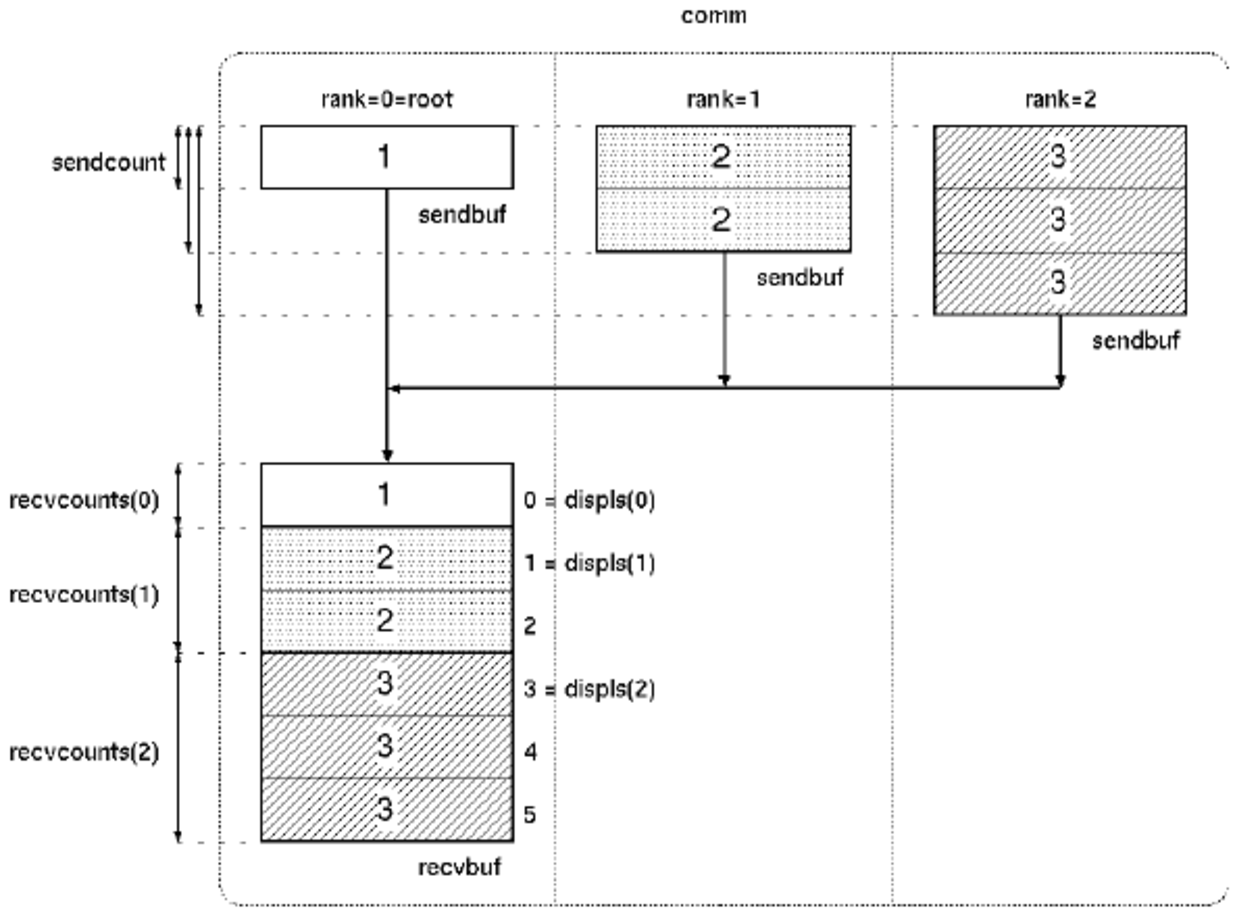
\includegraphics[scale=0.5]{03.MPI_Coll/gather2.pdf}
\end{frame}

\begin{frame}{Practicals}
    \begin{brown2block}{Exercise: 03.MPI\_Coll}
    \begin{enumerate}
        \setcounter{enumi}{1}
        \item Initialise an array and scatter it
    \end{enumerate}
    \end{brown2block}
\end{frame}


\subsection{All to all}
\begin{frame}[fragile]{Global exchange: All to All}
All-to-all communication: global exchange, all processes exchange their data. Useful for data transposition.\\
\begin{Fortranlisting}[]{}
CALL MPI_ALLTOALL(sndbuf, sndcount, sndtype,
                  rcvbuf, rcvcount, rcvtype, comm, ierr)
\end{Fortranlisting}
\begin{center}
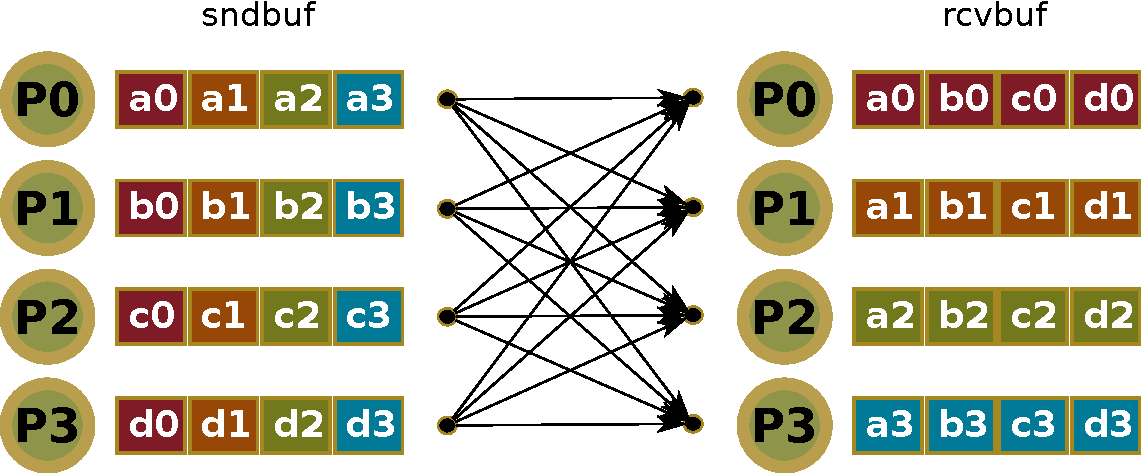
\includegraphics[scale=0.5]{03.MPI_Coll/alltoall.pdf}
\end{center}
\end{frame}


\subsection{Reduction}
\begin{frame}{Reduction}
The reduction operation allows to:
\begin{itemize}
\item Collect data from each process
\item Reduce the data to a single value
\item Store the result on the root processes
\item Store the result on all processes
\item Overlap communication and computation
\end{itemize}
\end{frame}

\begin{frame}[fragile]{Reduction}
\begin{Fortranlisting}[]{}
CALL MPI_REDUCE(sndbuf, rcvbuf, count, type, op,
                root, comm, ierr)
\end{Fortranlisting}
\begin{black1block}{}
\begin{tabular}{rp{8cm}}
\textbf{op} & (INTEGER) parallel operation to perform\\
\end{tabular}
\end{black1block}
\begin{center}
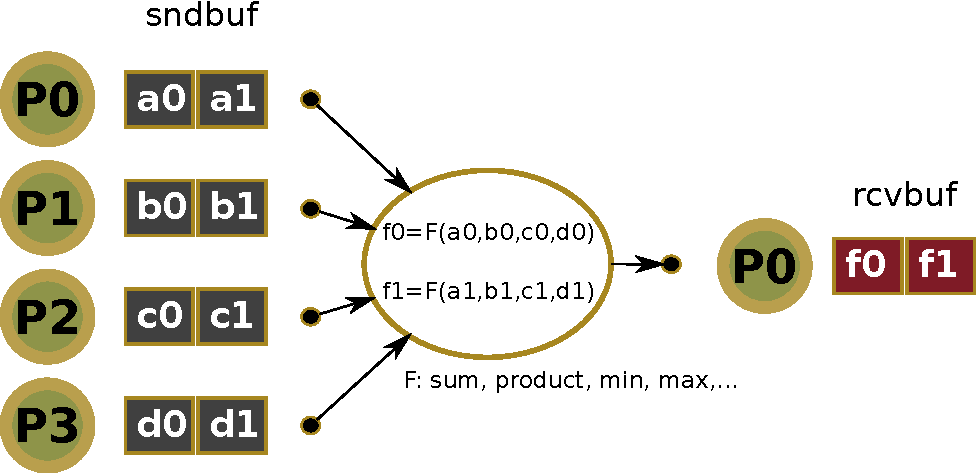
\includegraphics[scale=0.5]{03.MPI_Coll/reduce.pdf}
\end{center}
\end{frame}

\begin{frame}[fragile]{Reduction operators}
\begin{center}
\begin{tabular}{|c||c|}
    \hline
    \color{cscsblue}\textbf{MPI op} & \color{cscsbrown}\textbf{Operation} \\\hline\hline
    \verb+MPI_MAX+ & Maximum\\\hline
    \verb+MPI_MIN+ & Minimum\\\hline
    \verb+MPI_SUM+ & Sum\\\hline
    \verb+MPI_PROD+ & Product\\\hline
    \verb+MPI_LAND+ & Logical AND\\\hline
    \verb+MPI_BAND+ & Bitwise AND\\\hline
    \verb+MPI_LOR+ & Logical OR\\\hline
    \verb+MPI_BOR+ & Bitwise OR\\\hline
    \verb+MPI_LXOR+ & Logical exclusive OR\\\hline
    \verb+MPI_BXOR+ & Bitwise exclusive OR\\\hline
    \verb+MPI_MAXLOC+ & Maximum and location\\\hline
    \verb+MPI_MINLOC+ & Minimum and location\\\hline
\end{tabular}
\end{center}
\end{frame}

\subsection{Global collective operations}
\begin{frame}[fragile]{Global collective operations}
The result of the one-to-all operation is known by all ranks at the end of the operation.
\begin{Fortranlisting}[]{}
CALL MPI_ALLGATHER(sndbuf, sndcount, sndtype,
                   rcvbuf, rcvcount, rcvtype,
                   comm, ierr)

CALL MPI_ALLGATHERV(sndbuf, sndcount, sndtype,
                    rcvbuf, rcvcount, displs, rcvtype,
                    comm, ierr)

CALL MPI_ALLREDUCE(sndbuf, rcvbuf, count, type, op,
                   comm, ierr)
\end{Fortranlisting}
The argument \textbf{root} is missing, the result is stored in all processes.\\
\end{frame}

\subsection{Non-blocking coll-op}
\begin{frame}[fragile]{Non-blocking collective operations}
All collective operations have a non-blocking version.\\
Example:
\begin{Fortranlisting}[]{}
MPI_IBCAST(buf, count, type, root, comm, request, ierr)
\end{Fortranlisting}
Other functions:\\
\begin{Fortranlisting}[]{}
MPI_Iallgather, MPI_Iallgatherv, MPI_Iallreduce, MPI_Ialltoall
MPI_Ibarrier, MPI_Igather, MPI_Igatherv, MPI_Ireduce, MPI_Iscatter, MPI_Iscatterv
\end{Fortranlisting}
\end{frame}

\begin{frame}[fragile]{Other functions}
\begin{itemize}
    \item All-to-All operations, different buffer sizes and types:\\\hspace{1cm}\lstinlineCpp{MPI_AlltoAllv, MPI_AlltoAllw}
    \item Neighbor operations, based on topology:\\\hspace{1cm}\lstinlineCpp{MPI_Neighbor_gather, MPI_Neighbor_alltoall}
    \item Partial reduction:\\\hspace{1cm}\lstinlineCpp{MPI_Scan, MPI_Exscan}
    \item Create your own operator:\\\hspace{1cm}\lstinlineCpp{MPI_Op_create, MPI_Op_free}
    \item Reduce+Scatter:\\\hspace{1cm}\lstinlineCpp{MPI_Reduce_scatter, MPI_Reduce_scatter_block}
\end{itemize}
\end{frame}

\begin{frame}{Practicals}
    \begin{brown2block}{Exercise: 03.MPI\_Coll}
    \begin{enumerate}
        \setcounter{enumi}{2}
        \item Read data from the terminal and reduce
        \item Read data from the terminal and reduce if to all rank (allreduce)
    \end{enumerate}
    \end{brown2block}
\end{frame}

\section{Topology}
\section{Datatypes}

% THANK YOU SLIDE
\cscsthankyou{Thank you for your attention.}

\end{document}
